\section*{Introducci\'on}
El movimiento oscilatorio es un fenómeno presente es múltiples sistemas físicos, caracterizados
por incluir magnitudes que cambian periódicamente cerca de un punto de equilibrio estable.
En el mundo real, los sistemas oscilatorios tienen fuerzas disipativas que frenan las
oscilaciones, provocando que el sistema se detenga después de un cierto tiempo.

No obstante, es posible mantener las oscilaciones con una amplitud constante aplicando una
fuerza externa, denominada fuerza impulsora, que provee energía adicional para compensar la
perdida por el amortiguamiento. El movimiento que describe este sistema es de un
\textit{oscilador forzado} \cite{zemansky}, y es el tipo de oscilador más común en el mundo
real. La ecuación que describe el movimiento de un oscilador forzado es de la forma
\begin{equation}\label{eq:ecuaciongeneral}
	\dv[2]{x}{t} +2\gamma\dv{x}{t}+\omega_0^2x=F\cos(\omega_f t),
\end{equation}
donde $x$ es la posición del oscilador, $\gamma$ es la frecuencia de amortiguamiento,
$\omega_0$ es la frecuencia natural del sistema, $F$ es la amplitud de la fuerza impulsora
y $\omega_f$ es la frecuencia angular de la fuerza externa.

Una forma de controlar los parámetros de un oscilador forzado es mediante el péndulo de Pohl;
un péndulo de torsión constituido por un disco metálico acoplado a un resorte espiral, que oscila
alrededor del eje de simetría. Usando un electroimán y un motor, es posible controlar las
frecuencias $\gamma$ y $\omega_f$ respectivamente; en esencia, simulando las fuerzas
amortiguadoras e impulsoras del sistema. La Fig. (\ref{fig:POHL}) muestra un esquema del 
péndulo de Pohl con sus componentes más esenciales.
\begin{figure}[H]
	\centering
	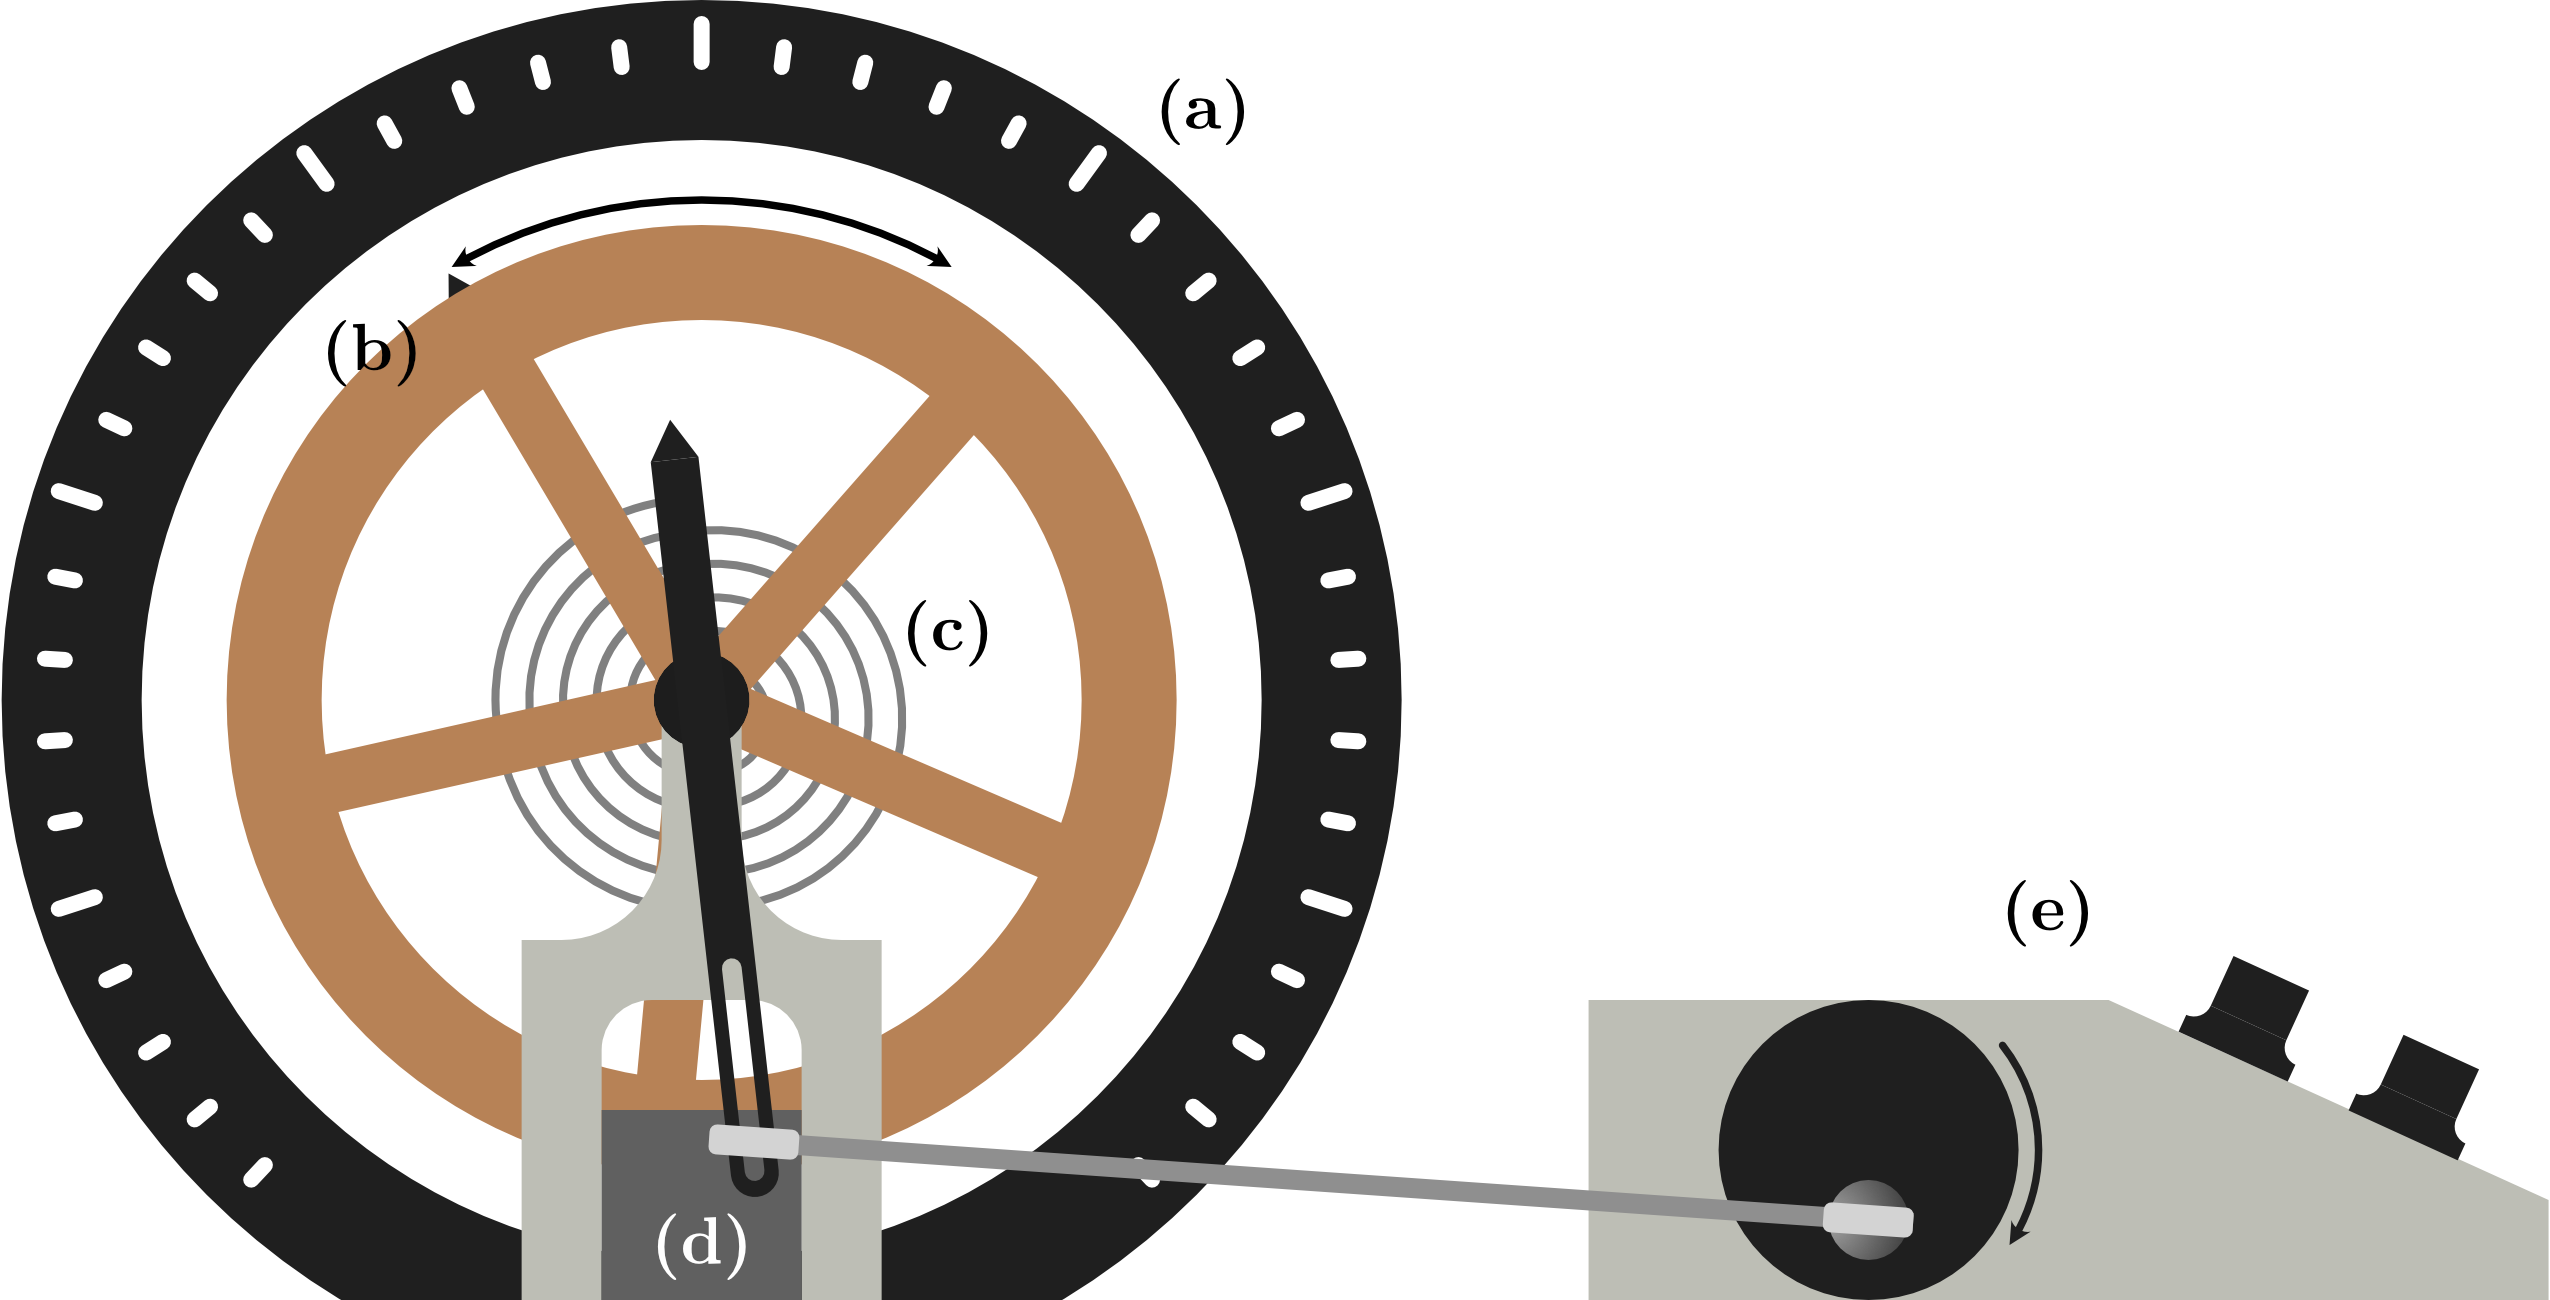
\includegraphics[width=\linewidth]{res/POHLFORZADO.png}
	\captionof{figure}{Péndulo de Pohl en movimiento. La rotación del motor impulsa las
		oscilaciones del péndulo.
		\textbf{(a)} escala de la amplitud del péndulo.
		\textbf{(b)} disco de cobre con indicador.
		\textbf{(c)} resorte helicoidal.
		\textbf{(d)} electroimán ajustable.
		\textbf{(e)} motor ajustable.}
	\label{fig:POHL}
\end{figure}
Considerando que la dinámica del disco de cobre puede ser descrita a través del torque ejercido
en él, la ecuación que describe su movimiento es de la forma
\begin{align}
	I\dv[2]{\theta}{t} &= -\kappa\theta - \lambda\dv{\theta}{t} + M_0\cos(\omega_f t) \nonumber \\
	\dv[2]{\theta}{t} + \frac{\lambda}{I}\dv{\theta}{t} + \frac{\kappa}{I}\theta &= \frac{M_0}{I}\cos(\omega_f t), \label{eq:ecuacionmov}
\end{align}
donde $\theta$ es el ángulo que hace el indicador del péndulo con el punto de equilibrio, $I$
es el momento de inercia del disco, $\kappa$ es la constante de torsión, $\lambda$ es el momento
de rozamiento y $M_0$ es la amplitud del momento forzado. Comparando los coeficientes de las
Ec. (\ref{eq:ecuaciongeneral}) y (\ref{eq:ecuacionmov}), se tiene que
\begin{align*}
	\gamma &= \frac{\lambda}{2I} \\
	\omega_0^2 &= \frac{\kappa}{I} \\
	F &= \frac{M_0}{I}.
\end{align*}

Ahora bien, dado que la ecuación de movimiento es una ecuación diferencial lineal, su solución
general, $\theta(t)$, está dada por la suma entre la solución de la ecuación homogénea, 
$\theta_H(t)$, y una solución particular, $\theta_P(t)$. La primera corresponde al movimiento
de un oscilador amortiguado no forzado
\begin{equation*}
	\theta_H(t) = Ae^{-\gamma t}\sin(\omega t +\varphi),
\end{equation*}
donde $A$ es la amplitud inicial, $\varphi$ es el desfase de la oscilación y $\omega$ es la
frecuencia amortiguada dada por
\begin{equation}
	\omega=\sqrt{\omega_0^2-\gamma^2}.
\end{equation}
Por otro lado, la segunda corresponde al \textit{estado estacionario} del movimiento; es decir,
cuando la única fuente de energía del sistema proviene de la fuerza impulsora
\begin{equation}\label{eq:solucionparticular}
	\theta_P(t) = A_M\cos(\omega_f t - \phi),
\end{equation}
donde $A_M$ es la amplitud de la oscilación forzada y $\phi$ es el desfase entre la fuerza
impulsora y la respuesta del oscilador dados por
\begin{align}
	A_M &= \frac{M_0/I}{\sqrt{\left(\omega_f^2 - \omega_0^2\right)^2 + 4\omega_f^2 \gamma^2}} \label{eq:amplitudforzada} \\
	\tan(\phi) &= \frac{2\gamma\omega_f}{\omega^2 - \omega_f^2}. \label{eq:desfaseforzado}
\end{align}

Existe un fenómeno particular propio de los osciladores forzados. Cuando la frecuencia de la
fuerza impulsora maximiza las oscilaciones del sistema, el oscilador entra en resonancia.
La frecuencia de resonancia, $\omega_R$, depende de las variables del sistema; específicamente
\begin{equation}\label{eq:frecuenciaresonancia}
	\omega_R = \sqrt{\omega_0^2 - 2\gamma^2}
\end{equation}

Con esto, es posible analizar el comportamiento del oscilador forzado y corroborar la
frecuencia de resonancia para un amortiguamiento dado. En ese sentido, en el presente informe
se determinó experimentalmente la frecuencia de resonancia del péndulo de Pohl para cuatro
amortiguamientos, con el fin de comprobar la relación entre la frecuencia de resonancia
$\omega_R$ y las constantes $\gamma$ y $\eval{A_M}_{\omega_f=\omega_R}$.

